% Options for packages loaded elsewhere
\PassOptionsToPackage{unicode}{hyperref}
\PassOptionsToPackage{hyphens}{url}
%
\documentclass[
]{article}
\usepackage{amsmath,amssymb}
\usepackage{lmodern}
\usepackage{iftex}
\ifPDFTeX
  \usepackage[T1]{fontenc}
  \usepackage[utf8]{inputenc}
  \usepackage{textcomp} % provide euro and other symbols
\else % if luatex or xetex
  \usepackage{unicode-math}
  \defaultfontfeatures{Scale=MatchLowercase}
  \defaultfontfeatures[\rmfamily]{Ligatures=TeX,Scale=1}
\fi
% Use upquote if available, for straight quotes in verbatim environments
\IfFileExists{upquote.sty}{\usepackage{upquote}}{}
\IfFileExists{microtype.sty}{% use microtype if available
  \usepackage[]{microtype}
  \UseMicrotypeSet[protrusion]{basicmath} % disable protrusion for tt fonts
}{}
\makeatletter
\@ifundefined{KOMAClassName}{% if non-KOMA class
  \IfFileExists{parskip.sty}{%
    \usepackage{parskip}
  }{% else
    \setlength{\parindent}{0pt}
    \setlength{\parskip}{6pt plus 2pt minus 1pt}}
}{% if KOMA class
  \KOMAoptions{parskip=half}}
\makeatother
\usepackage{xcolor}
\usepackage[margin=1in]{geometry}
\usepackage{color}
\usepackage{fancyvrb}
\newcommand{\VerbBar}{|}
\newcommand{\VERB}{\Verb[commandchars=\\\{\}]}
\DefineVerbatimEnvironment{Highlighting}{Verbatim}{commandchars=\\\{\}}
% Add ',fontsize=\small' for more characters per line
\usepackage{framed}
\definecolor{shadecolor}{RGB}{248,248,248}
\newenvironment{Shaded}{\begin{snugshade}}{\end{snugshade}}
\newcommand{\AlertTok}[1]{\textcolor[rgb]{0.94,0.16,0.16}{#1}}
\newcommand{\AnnotationTok}[1]{\textcolor[rgb]{0.56,0.35,0.01}{\textbf{\textit{#1}}}}
\newcommand{\AttributeTok}[1]{\textcolor[rgb]{0.77,0.63,0.00}{#1}}
\newcommand{\BaseNTok}[1]{\textcolor[rgb]{0.00,0.00,0.81}{#1}}
\newcommand{\BuiltInTok}[1]{#1}
\newcommand{\CharTok}[1]{\textcolor[rgb]{0.31,0.60,0.02}{#1}}
\newcommand{\CommentTok}[1]{\textcolor[rgb]{0.56,0.35,0.01}{\textit{#1}}}
\newcommand{\CommentVarTok}[1]{\textcolor[rgb]{0.56,0.35,0.01}{\textbf{\textit{#1}}}}
\newcommand{\ConstantTok}[1]{\textcolor[rgb]{0.00,0.00,0.00}{#1}}
\newcommand{\ControlFlowTok}[1]{\textcolor[rgb]{0.13,0.29,0.53}{\textbf{#1}}}
\newcommand{\DataTypeTok}[1]{\textcolor[rgb]{0.13,0.29,0.53}{#1}}
\newcommand{\DecValTok}[1]{\textcolor[rgb]{0.00,0.00,0.81}{#1}}
\newcommand{\DocumentationTok}[1]{\textcolor[rgb]{0.56,0.35,0.01}{\textbf{\textit{#1}}}}
\newcommand{\ErrorTok}[1]{\textcolor[rgb]{0.64,0.00,0.00}{\textbf{#1}}}
\newcommand{\ExtensionTok}[1]{#1}
\newcommand{\FloatTok}[1]{\textcolor[rgb]{0.00,0.00,0.81}{#1}}
\newcommand{\FunctionTok}[1]{\textcolor[rgb]{0.00,0.00,0.00}{#1}}
\newcommand{\ImportTok}[1]{#1}
\newcommand{\InformationTok}[1]{\textcolor[rgb]{0.56,0.35,0.01}{\textbf{\textit{#1}}}}
\newcommand{\KeywordTok}[1]{\textcolor[rgb]{0.13,0.29,0.53}{\textbf{#1}}}
\newcommand{\NormalTok}[1]{#1}
\newcommand{\OperatorTok}[1]{\textcolor[rgb]{0.81,0.36,0.00}{\textbf{#1}}}
\newcommand{\OtherTok}[1]{\textcolor[rgb]{0.56,0.35,0.01}{#1}}
\newcommand{\PreprocessorTok}[1]{\textcolor[rgb]{0.56,0.35,0.01}{\textit{#1}}}
\newcommand{\RegionMarkerTok}[1]{#1}
\newcommand{\SpecialCharTok}[1]{\textcolor[rgb]{0.00,0.00,0.00}{#1}}
\newcommand{\SpecialStringTok}[1]{\textcolor[rgb]{0.31,0.60,0.02}{#1}}
\newcommand{\StringTok}[1]{\textcolor[rgb]{0.31,0.60,0.02}{#1}}
\newcommand{\VariableTok}[1]{\textcolor[rgb]{0.00,0.00,0.00}{#1}}
\newcommand{\VerbatimStringTok}[1]{\textcolor[rgb]{0.31,0.60,0.02}{#1}}
\newcommand{\WarningTok}[1]{\textcolor[rgb]{0.56,0.35,0.01}{\textbf{\textit{#1}}}}
\usepackage{graphicx}
\makeatletter
\def\maxwidth{\ifdim\Gin@nat@width>\linewidth\linewidth\else\Gin@nat@width\fi}
\def\maxheight{\ifdim\Gin@nat@height>\textheight\textheight\else\Gin@nat@height\fi}
\makeatother
% Scale images if necessary, so that they will not overflow the page
% margins by default, and it is still possible to overwrite the defaults
% using explicit options in \includegraphics[width, height, ...]{}
\setkeys{Gin}{width=\maxwidth,height=\maxheight,keepaspectratio}
% Set default figure placement to htbp
\makeatletter
\def\fps@figure{htbp}
\makeatother
\setlength{\emergencystretch}{3em} % prevent overfull lines
\providecommand{\tightlist}{%
  \setlength{\itemsep}{0pt}\setlength{\parskip}{0pt}}
\setcounter{secnumdepth}{-\maxdimen} % remove section numbering
\usepackage{xeCJK}
\ifLuaTeX
  \usepackage{selnolig}  % disable illegal ligatures
\fi
\IfFileExists{bookmark.sty}{\usepackage{bookmark}}{\usepackage{hyperref}}
\IfFileExists{xurl.sty}{\usepackage{xurl}}{} % add URL line breaks if available
\urlstyle{same} % disable monospaced font for URLs
\hypersetup{
  hidelinks,
  pdfcreator={LaTeX via pandoc}}

\author{}
\date{\vspace{-2.5em}}

\begin{document}

\hypertarget{biostatistics-homework-7}{%
\section{Biostatistics Homework 7}\label{biostatistics-homework-7}}

By \(\mathbb{L}\)umi (张鹿鸣12112618)

\vspace{5mm}

\hypertarget{vaccine}{%
\subsection{1. Vaccine}\label{vaccine}}

\hypertarget{section}{%
\subsubsection{1.1)}\label{section}}

TFTFTFFFT

I'm wondering, the ARV/ARU ratio should also be the odds ratio of
vaccination among the people who get the disease right?

I think it's right.

\hypertarget{section-1}{%
\subsubsection{1.2)}\label{section-1}}

\begin{Shaded}
\begin{Highlighting}[]
\FunctionTok{data.frame}\NormalTok{(}
  \StringTok{\textasciigrave{}}\AttributeTok{mRNA{-}1273}\StringTok{\textasciigrave{}} \OtherTok{=} \FunctionTok{c}\NormalTok{(}\DecValTok{11}\NormalTok{, }\DecValTok{15181} \SpecialCharTok{{-}} \DecValTok{11}\NormalTok{, }\DecValTok{15181}\NormalTok{),}
  \AttributeTok{Placebo =} \FunctionTok{c}\NormalTok{(}\DecValTok{185}\NormalTok{, }\DecValTok{15170} \SpecialCharTok{{-}} \DecValTok{185}\NormalTok{, }\DecValTok{15170}\NormalTok{),}
  \AttributeTok{Total =} \FunctionTok{c}\NormalTok{(}\DecValTok{11} \SpecialCharTok{+} \DecValTok{185}\NormalTok{, }\DecValTok{15181} \SpecialCharTok{+} \DecValTok{15170} \SpecialCharTok{{-}} \DecValTok{11} \SpecialCharTok{{-}} \DecValTok{185}\NormalTok{, }\DecValTok{15181} \SpecialCharTok{+} \DecValTok{15170}\NormalTok{),}
  \AttributeTok{row.names =} \FunctionTok{c}\NormalTok{(}\StringTok{"COVID 19"}\NormalTok{, }\StringTok{"No Symptoms"}\NormalTok{, }\StringTok{"Total"}\NormalTok{)}
\NormalTok{)}
\end{Highlighting}
\end{Shaded}

\begin{verbatim}
##             mRNA.1273 Placebo Total
## COVID 19           11     185   196
## No Symptoms     15170   14985 30155
## Total           15181   15170 30351
\end{verbatim}

\hypertarget{section-2}{%
\subsubsection{1.3)}\label{section-2}}

From 1.1, we know that

\[
\text{vaccine efficacy} = (1 - \frac{ARV}{ARU}) \times 100\%
\]

Thus the vaccine efficacy for our mRNA vaccine is:

\[
\text{vaccine efficacy}_\text{mRNA} = (1 - \frac{11 / 15181}{185 / 15170} ) \times 100\% \approx 94.06%
\]

\hypertarget{section-3}{%
\subsubsection{1.4)}\label{section-3}}

\(H_0\): Vaccination and infection status are independent.

\(H_1\): Vaccination and infection status are not independent.

For the expected values in the table, I will just list an equation here
and ignore the calculations. Suppose \(e_{ij}\) is the expected value on
the \(i\)th row and \(j\)th column:

\[
e_{ij} = \frac{\sum_{k = 1}^i a_{kj}}{\sum_{m=1}^i \sum_{n=1}^j a_{mn}}\times \sum_{k=1}^j a_{ik}
\]

R helped me to calculate the table, which is the output of the following
code:

\begin{Shaded}
\begin{Highlighting}[]
\NormalTok{vaccine }\OtherTok{\textless{}{-}} \FunctionTok{data.frame}\NormalTok{(}
  \StringTok{\textasciigrave{}}\AttributeTok{mRNA{-}1273}\StringTok{\textasciigrave{}} \OtherTok{=} \FunctionTok{c}\NormalTok{(}\DecValTok{11}\NormalTok{, }\DecValTok{15181} \SpecialCharTok{{-}} \DecValTok{11}\NormalTok{),}
  \AttributeTok{Placebo =} \FunctionTok{c}\NormalTok{(}\DecValTok{185}\NormalTok{, }\DecValTok{15170} \SpecialCharTok{{-}} \DecValTok{185}\NormalTok{),}
  \AttributeTok{row.names =} \FunctionTok{c}\NormalTok{(}\StringTok{"COVID 19"}\NormalTok{, }\StringTok{"No Symptoms"}\NormalTok{)}
\NormalTok{)}
\NormalTok{chisq\_vaccine }\OtherTok{\textless{}{-}} \FunctionTok{chisq.test}\NormalTok{(vaccine)}
\NormalTok{chisq\_vaccine}\SpecialCharTok{$}\NormalTok{expected}
\end{Highlighting}
\end{Shaded}

\begin{verbatim}
##               mRNA.1273     Placebo
## COVID 19       98.03552    97.96448
## No Symptoms 15082.96448 15072.03552
\end{verbatim}

\begin{Shaded}
\begin{Highlighting}[]
\NormalTok{chisq\_vaccine}
\end{Highlighting}
\end{Shaded}

\begin{verbatim}
## 
##  Pearson's Chi-squared test with Yates' continuity correction
## 
## data:  vaccine
## X-squared = 153.82, df = 1, p-value < 2.2e-16
\end{verbatim}

As we can see, the \(\chi^2\) score is extremely high (153.8177), and
thus the adjusted p-value is extremely low, \(2.538393\times10^{-35}\)
to be more preciese.

Here we performed a continuity correction, if we didn't perform the
correction, the p-value and statistics should be:

\begin{Shaded}
\begin{Highlighting}[]
\FunctionTok{chisq.test}\NormalTok{(vaccine, }\AttributeTok{correct =}\NormalTok{ F)}
\end{Highlighting}
\end{Shaded}

\begin{verbatim}
## 
##  Pearson's Chi-squared test
## 
## data:  vaccine
## X-squared = 155.6, df = 1, p-value < 2.2e-16
\end{verbatim}

The uncorrected p-value is \(1.035122\times 10^{-35}\), which is also
very small.

\hypertarget{section-4}{%
\subsubsection{1.5)}\label{section-4}}

First we should ensure that our samples are randomly selected and that
they are independent from each other.

Then, we should make sure that the number in all the cells are larger
than ten, so that we can approximate the binomial distribution to a
normal distribution.

\hypertarget{using-effect-size-too}{%
\subsection{2. Using Effect Size Too}\label{using-effect-size-too}}

\hypertarget{section-5}{%
\subsubsection{2.1)}\label{section-5}}

A wrong interpretation:

From the paper, we can know that if we would like to use the Cohen's
\(d\) to calculate the effect size, then:

\[
d = \frac{M_1 - M_0}{s}
\]

Where \(M_1\) and \(M_0\) are the mean of the two groups. \(s\) is the
standard deviation of either groups.

The table we are using:

\begin{Shaded}
\begin{Highlighting}[]
\NormalTok{blood }\OtherTok{\textless{}{-}} \FunctionTok{data.frame}\NormalTok{(}
  \AttributeTok{A =} \FunctionTok{c}\NormalTok{(}\DecValTok{1188}\NormalTok{, }\DecValTok{670}\NormalTok{),}
  \StringTok{\textasciigrave{}}\AttributeTok{Non{-}A}\StringTok{\textasciigrave{}} \OtherTok{=} \FunctionTok{c}\NormalTok{(}\DecValTok{2506}\NormalTok{, }\DecValTok{1105}\NormalTok{),}
  \AttributeTok{row.names =} \FunctionTok{c}\NormalTok{(}\StringTok{"Healthy"}\NormalTok{, }\StringTok{"COVID{-}19"}\NormalTok{)}
\NormalTok{)}
\NormalTok{blood}
\end{Highlighting}
\end{Shaded}

\begin{verbatim}
##             A Non.A
## Healthy  1188  2506
## COVID-19  670  1105
\end{verbatim}

\begin{Shaded}
\begin{Highlighting}[]
\NormalTok{mean\_A }\OtherTok{\textless{}{-}} \FunctionTok{mean}\NormalTok{(blood[,}\DecValTok{1}\NormalTok{])}
\NormalTok{mean\_nonA }\OtherTok{\textless{}{-}} \FunctionTok{mean}\NormalTok{(blood[,}\DecValTok{2}\NormalTok{])}
\NormalTok{sd\_A }\OtherTok{\textless{}{-}} \FunctionTok{sd}\NormalTok{(blood[,}\DecValTok{1}\NormalTok{])}
\NormalTok{eff }\OtherTok{\textless{}{-}}\NormalTok{ (mean\_A }\SpecialCharTok{{-}}\NormalTok{ mean\_nonA) }\SpecialCharTok{/}\NormalTok{ sd\_A}
\NormalTok{eff}
\end{Highlighting}
\end{Shaded}

\begin{verbatim}
## [1] -2.392969
\end{verbatim}

The correct interpretation:

I don't think it's that right. Since the mean number in A and nonA don't
have a real meaning. I googled it again and Google told me that it is
best to use the odds ratio for a 2 by 2 contingency tables. I think I
misunderstood the article. Well, maybe we should calculate it again.

\[
OR = \frac{ad}{bc} = \frac{2506 \times 670}{1188 \times 1105} \approx 1.279
\]

In this case, the diseased are considered the event of interest.

\hypertarget{section-6}{%
\subsubsection{2.2)}\label{section-6}}

D

\hypertarget{section-7}{%
\subsubsection{2.3)}\label{section-7}}

The effect size in the first problem can be calculated by:

\[
OR = \frac{\text{COVID}_\text{vaccine} \times \text{no COVID}_\text{no vaccine}}{\text{COVID}_\text{no vaccine} \times \text{no COVID}_\text{vaccine}} = \frac{11 \times 14985}{185 \times 15170} = 0.0587
\]

Which is quite small, indicating that taking the vaccine might have a
huge impact getting COVID. The RNA vaccine really lowers the odds of
getting COVID.

\hypertarget{section-8}{%
\subsubsection{2.4)}\label{section-8}}

The effect size tell us in a normalized scale how much the value in your
experiment group differs from the control group. We should care about it
because p-values only tell us how significant something is going to
happen, but we cannot directly see the difference quantitatively. It
might be very significant due to a very large sample size, while the
actual difference between the two groups are small.

\hypertarget{the-white-stock}{%
\subsection{3. The White Stock}\label{the-white-stock}}

\hypertarget{section-9}{%
\subsubsection{3.1)}\label{section-9}}

i.

The equation for Pearson's Correlation Coefficient is:

\[
r = \frac{\sigma(X, Y)}{\sqrt{\text{Var}(X) \text{Var}(Y)}}
\]

\begin{Shaded}
\begin{Highlighting}[]
\NormalTok{stork }\OtherTok{\textless{}{-}} \FunctionTok{data.frame}\NormalTok{(}
  \AttributeTok{Storks =} \FunctionTok{c}\NormalTok{(}\DecValTok{100}\NormalTok{,}\DecValTok{300}\NormalTok{,}\DecValTok{1}\NormalTok{,}\DecValTok{5000}\NormalTok{,}\DecValTok{9}\NormalTok{,}\DecValTok{140}\NormalTok{,}\DecValTok{3300}\NormalTok{,}\DecValTok{2500}\NormalTok{,}\DecValTok{4}\NormalTok{,}\DecValTok{5000}\NormalTok{,}\DecValTok{5}\NormalTok{,}\DecValTok{30000}\NormalTok{,}\DecValTok{1500}\NormalTok{,}\DecValTok{5000}\NormalTok{,}\DecValTok{8000}\NormalTok{,}\DecValTok{150}\NormalTok{,}\DecValTok{25000}\NormalTok{),}
  \AttributeTok{Birth\_rate =} \FunctionTok{c}\NormalTok{(}\DecValTok{83}\NormalTok{,}\DecValTok{87}\NormalTok{,}\DecValTok{118}\NormalTok{,}\DecValTok{117}\NormalTok{,}\DecValTok{59}\NormalTok{,}\DecValTok{774}\NormalTok{,}\DecValTok{901}\NormalTok{,}\DecValTok{106}\NormalTok{,}\DecValTok{188}\NormalTok{,}\DecValTok{124}\NormalTok{,}\DecValTok{551}\NormalTok{,}\DecValTok{610}\NormalTok{,}\DecValTok{120}\NormalTok{,}\DecValTok{367}\NormalTok{,}\DecValTok{439}\NormalTok{,}\DecValTok{82}\NormalTok{,}\DecValTok{1576}\NormalTok{)}
\NormalTok{)}
\NormalTok{r }\OtherTok{\textless{}{-}} \FunctionTok{cov}\NormalTok{(stork}\SpecialCharTok{$}\NormalTok{Storks, stork}\SpecialCharTok{$}\NormalTok{Birth\_rate) }\SpecialCharTok{/} \FunctionTok{sqrt}\NormalTok{(}\FunctionTok{var}\NormalTok{(stork}\SpecialCharTok{$}\NormalTok{Storks) }\SpecialCharTok{*} \FunctionTok{var}\NormalTok{(stork}\SpecialCharTok{$}\NormalTok{Birth\_rate))}
\NormalTok{r}
\end{Highlighting}
\end{Shaded}

\begin{verbatim}
## [1] 0.6202653
\end{verbatim}

Here we directly used the R function to calculate the covariance, which
is

\begin{Shaded}
\begin{Highlighting}[]
\FunctionTok{cov}\NormalTok{(stork}\SpecialCharTok{$}\NormalTok{Storks, stork}\SpecialCharTok{$}\NormalTok{Birth\_rate)}
\end{Highlighting}
\end{Shaded}

\begin{verbatim}
## [1] 2246592
\end{verbatim}

We can also calculate the covariance using the formula:

\[
\sigma(X,Y) = E(XY) - E(X)E(Y)
\]

Which gives us:

\begin{Shaded}
\begin{Highlighting}[]
\FunctionTok{mean}\NormalTok{(stork}\SpecialCharTok{$}\NormalTok{Storks }\SpecialCharTok{*}\NormalTok{ stork}\SpecialCharTok{$}\NormalTok{Birth\_rate) }\SpecialCharTok{{-}} \FunctionTok{mean}\NormalTok{(stork}\SpecialCharTok{$}\NormalTok{Storks) }\SpecialCharTok{*} \FunctionTok{mean}\NormalTok{(stork}\SpecialCharTok{$}\NormalTok{Birth\_rate)}
\end{Highlighting}
\end{Shaded}

\begin{verbatim}
## [1] 2114440
\end{verbatim}

Which is different because R function cov() uses a different formula:

\[
\sigma(X,Y) = \frac{\sum(x_i - \bar x)(y_i - \bar y)}{n-1}
\]

So we should do some adjustments:

\begin{Shaded}
\begin{Highlighting}[]
\NormalTok{n }\OtherTok{\textless{}{-}} \FunctionTok{length}\NormalTok{(stork}\SpecialCharTok{$}\NormalTok{Storks)}
\NormalTok{(}\FunctionTok{mean}\NormalTok{(stork}\SpecialCharTok{$}\NormalTok{Storks }\SpecialCharTok{*}\NormalTok{ stork}\SpecialCharTok{$}\NormalTok{Birth\_rate) }\SpecialCharTok{{-}} \FunctionTok{mean}\NormalTok{(stork}\SpecialCharTok{$}\NormalTok{Storks) }\SpecialCharTok{*} \FunctionTok{mean}\NormalTok{(stork}\SpecialCharTok{$}\NormalTok{Birth\_rate)) }\SpecialCharTok{*}\NormalTok{ n }\SpecialCharTok{/}\NormalTok{ (n }\SpecialCharTok{{-}} \DecValTok{1}\NormalTok{)}
\end{Highlighting}
\end{Shaded}

\begin{verbatim}
## [1] 2246592
\end{verbatim}

Now it's the same.

The Pearson correlation coefficient is 0.6202.

\begin{enumerate}
\def\labelenumi{\roman{enumi})}
\setcounter{enumi}{1}
\tightlist
\item
\end{enumerate}

Based on the correlation coefficient, there is a positive linear
relationship between the Storks(pairs) and Birth rate (\(10^3\)/yr) .

\begin{enumerate}
\def\labelenumi{\roman{enumi})}
\setcounter{enumi}{2}
\tightlist
\item
\end{enumerate}

We can calculate a t-score based on the correlation coefficient.

\[
t = r \cdot \sqrt{\frac{n - 2}{1-r^2}} \sim T(n-2)
\]

Where \(n\) is the number of samples. So our t-score is,

\[
t = 0.6202 \times\sqrt{\frac{17 - 2}{1 - 0.6202^2}} \approx 3.062
\]

And the corresponding p-value:

\begin{Shaded}
\begin{Highlighting}[]
\FunctionTok{pt}\NormalTok{(}\FloatTok{3.062}\NormalTok{, }\DecValTok{15}\NormalTok{, }\AttributeTok{lower.tail =}\NormalTok{ F) }\SpecialCharTok{*} \DecValTok{2}
\end{Highlighting}
\end{Shaded}

\begin{verbatim}
## [1] 0.007907499
\end{verbatim}

\begin{enumerate}
\def\labelenumi{\roman{enumi})}
\setcounter{enumi}{3}
\tightlist
\item
\end{enumerate}

For a simple linear regression using OLS,

\[
a = \frac{\sigma(X,Y)}{\text{Var}(X)}, b = \bar y - a \bar x
\]

So based on our previous answers, if we use our own calculation of
covariance:

\begin{Shaded}
\begin{Highlighting}[]
\NormalTok{a\_adjust }\OtherTok{\textless{}{-}} \DecValTok{2114440} \SpecialCharTok{/} \FunctionTok{var}\NormalTok{(stork}\SpecialCharTok{$}\NormalTok{Storks)}
\NormalTok{b\_adjust }\OtherTok{\textless{}{-}} \FunctionTok{mean}\NormalTok{(stork}\SpecialCharTok{$}\NormalTok{Birth\_rate) }\SpecialCharTok{{-}}\NormalTok{ a\_adjust }\SpecialCharTok{*} \FunctionTok{mean}\NormalTok{(stork}\SpecialCharTok{$}\NormalTok{Storks)}
\FunctionTok{c}\NormalTok{(a\_adjust, b\_adjust)}
\end{Highlighting}
\end{Shaded}

\begin{verbatim}
## [1]   0.0270999 233.5979093
\end{verbatim}

If we use R's calculation of the covariance:

\begin{Shaded}
\begin{Highlighting}[]
\NormalTok{a }\OtherTok{\textless{}{-}} \DecValTok{2246592} \SpecialCharTok{/} \FunctionTok{var}\NormalTok{(stork}\SpecialCharTok{$}\NormalTok{Storks)}
\NormalTok{b }\OtherTok{\textless{}{-}} \FunctionTok{mean}\NormalTok{(stork}\SpecialCharTok{$}\NormalTok{Birth\_rate) }\SpecialCharTok{{-}}\NormalTok{ a }\SpecialCharTok{*} \FunctionTok{mean}\NormalTok{(stork}\SpecialCharTok{$}\NormalTok{Storks)}
\FunctionTok{c}\NormalTok{(a, b)}
\end{Highlighting}
\end{Shaded}

\begin{verbatim}
## [1]   0.02879364 225.02869336
\end{verbatim}

We can also use R's function to calculate the slope and intersection:

\begin{Shaded}
\begin{Highlighting}[]
\NormalTok{model }\OtherTok{\textless{}{-}} \FunctionTok{lm}\NormalTok{(stork}\SpecialCharTok{$}\NormalTok{Birth\_rate }\SpecialCharTok{\textasciitilde{}}\NormalTok{ stork}\SpecialCharTok{$}\NormalTok{Storks)}
\NormalTok{model}
\end{Highlighting}
\end{Shaded}

\begin{verbatim}
## 
## Call:
## lm(formula = stork$Birth_rate ~ stork$Storks)
## 
## Coefficients:
##  (Intercept)  stork$Storks  
##    225.02869       0.02879
\end{verbatim}

\begin{enumerate}
\def\labelenumi{\alph{enumi})}
\setcounter{enumi}{21}
\tightlist
\item
\end{enumerate}

There is a difference between the ways you calculate the covariance.
Because we are calculating the covariance of a sample, we need to follow
the formula
\(\sigma(X,Y) = \frac{\sum(x_i - \bar x)(y_i - \bar y)}{n-1}\), instead
of \(E(XY) - E(X) E(Y)\). Since the population mean is unknown, and one
degree of freedom is used to estimate \(\bar x\) and \(\bar y\).

\hypertarget{section-10}{%
\subsubsection{3.2)}\label{section-10}}

So, if we want to see the correlation between area and birth rate:

\begin{Shaded}
\begin{Highlighting}[]
\NormalTok{area }\OtherTok{\textless{}{-}} \FunctionTok{data.frame}\NormalTok{(}
  \AttributeTok{Area =} \FunctionTok{c}\NormalTok{(}\DecValTok{28750}\NormalTok{,}\DecValTok{83860}\NormalTok{,}\DecValTok{30520}\NormalTok{,}\DecValTok{111000}\NormalTok{,}\DecValTok{43100}\NormalTok{,}\DecValTok{544000}\NormalTok{,}\DecValTok{357000}\NormalTok{,}\DecValTok{132000}\NormalTok{,}
           \DecValTok{41900}\NormalTok{,}\DecValTok{93000}\NormalTok{,}\DecValTok{301280}\NormalTok{,}\DecValTok{312680}\NormalTok{,}\DecValTok{92390}\NormalTok{,}\DecValTok{237500}\NormalTok{,}\DecValTok{504750}\NormalTok{,}\DecValTok{41290}\NormalTok{,}\DecValTok{779450}\NormalTok{),}
  \AttributeTok{Birth\_rate =} \FunctionTok{c}\NormalTok{(}\DecValTok{83}\NormalTok{,}\DecValTok{87}\NormalTok{,}\DecValTok{118}\NormalTok{,}\DecValTok{117}\NormalTok{,}\DecValTok{59}\NormalTok{,}\DecValTok{774}\NormalTok{,}\DecValTok{901}\NormalTok{,}\DecValTok{106}\NormalTok{,}\DecValTok{188}\NormalTok{,}\DecValTok{124}\NormalTok{,}\DecValTok{551}\NormalTok{,}\DecValTok{610}\NormalTok{,}\DecValTok{120}\NormalTok{,}\DecValTok{367}\NormalTok{,}\DecValTok{439}\NormalTok{,}\DecValTok{82}\NormalTok{,}\DecValTok{1576}\NormalTok{)}
\NormalTok{)}
\NormalTok{r\_area }\OtherTok{\textless{}{-}} \FunctionTok{cov}\NormalTok{(area}\SpecialCharTok{$}\NormalTok{Area, area}\SpecialCharTok{$}\NormalTok{Birth\_rate) }\SpecialCharTok{/} \FunctionTok{sqrt}\NormalTok{(}\FunctionTok{var}\NormalTok{(area}\SpecialCharTok{$}\NormalTok{Area) }\SpecialCharTok{*} \FunctionTok{var}\NormalTok{(area}\SpecialCharTok{$}\NormalTok{Birth\_rate))}
\NormalTok{r\_area}
\end{Highlighting}
\end{Shaded}

\begin{verbatim}
## [1] 0.9225445
\end{verbatim}

As we can see, the pearson correlation coefficient of area and birth
rate is 0.9225, which is pretty high. Indicating there is a positive
linear relationship between the area of the country and the birth rate.

We can also calculate the t-score:

\[
t = r \cdot \sqrt{\frac{n - 2}{ 1 - r^2}} = 0.9225 \times \sqrt{\frac{17 - 2}{1 - 0.9225^2}} \approx 9.2591
\]

\begin{Shaded}
\begin{Highlighting}[]
\FunctionTok{pt}\NormalTok{(}\FloatTok{9.2591}\NormalTok{, }\DecValTok{15}\NormalTok{, }\AttributeTok{lower.tail =}\NormalTok{ F) }\SpecialCharTok{*} \DecValTok{2}
\end{Highlighting}
\end{Shaded}

\begin{verbatim}
## [1] 1.362273e-07
\end{verbatim}

The p-value is \(1.362 \times 10^{-7}\), which is extremely small.

\begin{Shaded}
\begin{Highlighting}[]
\FunctionTok{lm}\NormalTok{(area}\SpecialCharTok{$}\NormalTok{Area }\SpecialCharTok{\textasciitilde{}}\NormalTok{ area}\SpecialCharTok{$}\NormalTok{Birth\_rate)}
\end{Highlighting}
\end{Shaded}

\begin{verbatim}
## 
## Call:
## lm(formula = area$Area ~ area$Birth_rate)
## 
## Coefficients:
##     (Intercept)  area$Birth_rate  
##           36553              494
\end{verbatim}

The coefficients for the simple linear regression are slope = 494,
intercept = 36553. As we can see from the plot below, the function fits
quite well.

\begin{Shaded}
\begin{Highlighting}[]
\FunctionTok{ggplot}\NormalTok{(}\AttributeTok{data =}\NormalTok{ area, }\AttributeTok{mapping =} \FunctionTok{aes}\NormalTok{(Birth\_rate, Area)) }\SpecialCharTok{+} 
  \FunctionTok{geom\_point}\NormalTok{() }\SpecialCharTok{+} 
  \FunctionTok{geom\_abline}\NormalTok{(}\AttributeTok{slope =} \DecValTok{494}\NormalTok{, }\AttributeTok{intercept =} \DecValTok{36553}\NormalTok{, }\AttributeTok{colour =} \StringTok{"red"}\NormalTok{)}
\end{Highlighting}
\end{Shaded}

\begin{center}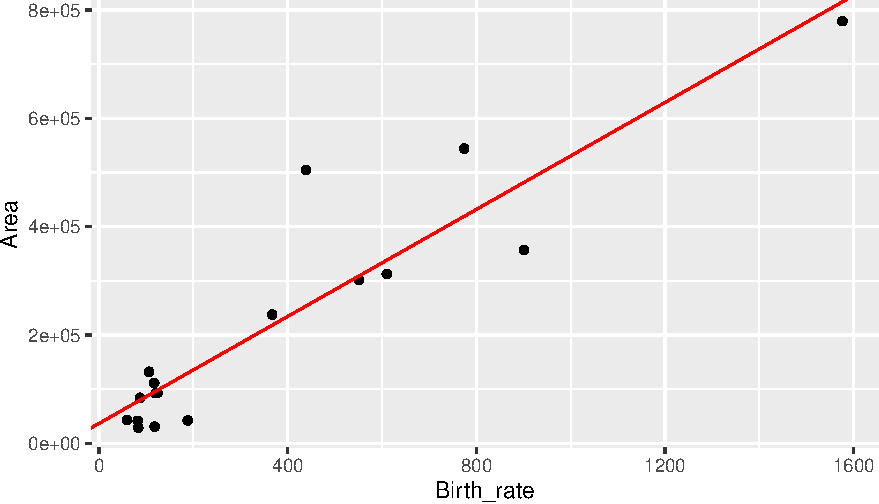
\includegraphics{Homework7_files/figure-latex/unnamed-chunk-18-1} \end{center}

\hypertarget{section-11}{%
\subsubsection{3.3)}\label{section-11}}

We might need to perform another correlation check between the area and
the amount of Storks.

\begin{Shaded}
\begin{Highlighting}[]
\FunctionTok{cor}\NormalTok{(area}\SpecialCharTok{$}\NormalTok{Area, stork}\SpecialCharTok{$}\NormalTok{Storks)}
\end{Highlighting}
\end{Shaded}

\begin{verbatim}
## [1] 0.5793423
\end{verbatim}

We can see there is a slightly positive correlation between the land
area of the country and the number of storks observed in that country.

\begin{Shaded}
\begin{Highlighting}[]
\NormalTok{area\_stork }\OtherTok{\textless{}{-}} \FunctionTok{lm}\NormalTok{(area}\SpecialCharTok{$}\NormalTok{Area }\SpecialCharTok{\textasciitilde{}}\NormalTok{ stork}\SpecialCharTok{$}\NormalTok{Storks)}
\FunctionTok{ggplot}\NormalTok{(}\AttributeTok{mapping =} \FunctionTok{aes}\NormalTok{(stork}\SpecialCharTok{$}\NormalTok{Storks,area}\SpecialCharTok{$}\NormalTok{Area)) }\SpecialCharTok{+} 
  \FunctionTok{geom\_point}\NormalTok{() }\SpecialCharTok{+} \FunctionTok{xlab}\NormalTok{(}\StringTok{\textquotesingle{}Storks\textquotesingle{}}\NormalTok{) }\SpecialCharTok{+} \FunctionTok{ylab}\NormalTok{(}\StringTok{\textquotesingle{}Area\textquotesingle{}}\NormalTok{) }\SpecialCharTok{+}
  \FunctionTok{geom\_abline}\NormalTok{(}\AttributeTok{slope =} \FunctionTok{coef}\NormalTok{(area\_stork)[}\DecValTok{2}\NormalTok{], }\AttributeTok{intercept =} \FunctionTok{coef}\NormalTok{(area\_stork)[}\DecValTok{1}\NormalTok{], }\AttributeTok{colour =} \StringTok{\textquotesingle{}red\textquotesingle{}}\NormalTok{)}
\end{Highlighting}
\end{Shaded}

\begin{center}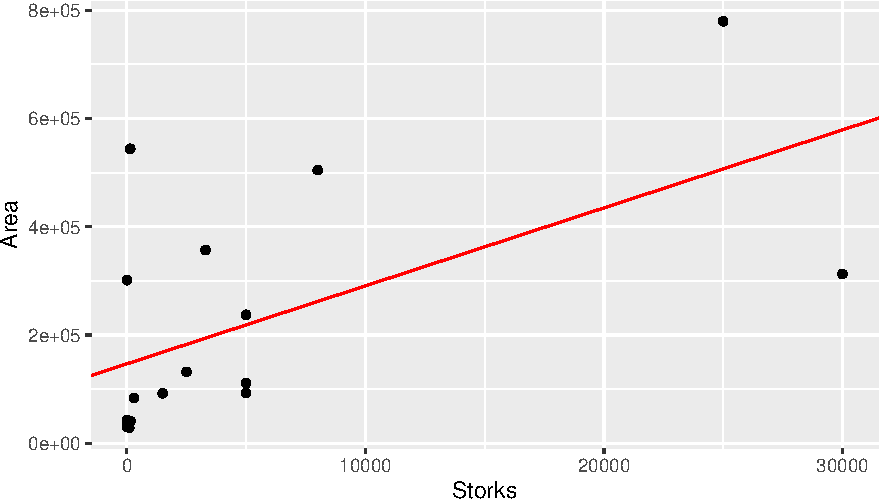
\includegraphics{Homework7_files/figure-latex/unnamed-chunk-20-1} \end{center}

With the very strong correlation between the birth rate and country
size, the not-so-strong correlation of stork numbers and country size
might be amplified, resulting in a strong correlation between the stork
population and birth rate.

\hypertarget{section-12}{%
\subsubsection{3.4)}\label{section-12}}

As described in 3.3), the confounding variable in this study might be
the area of the country. Which is reasonable. The larger the country,
the more birds it might ``contain'', and it have a larger birth rate
since they might have a larger population.

Thus, the area and both stork population and birth rate have positive
correlations. Leading to a misjudgment. I don't know if China have these
lot storks, so if we include some Asian countries, like China or India,
this correlation might not be that obvious.

\end{document}
